\chapter{Introduction}

%The story  I want to tell explains the Casimir force via its historical origins which serve to introduce the big results,
% while sidestepping weird irrelevant bullshit.
%  I want to hit the important context for modern scientists and emphasize quantities realted to current experiments.
%  I also want to outline the currently available most powerful methods to set context for what else is possible,
% and what its limitations are.  

%I think I can do this with a partial historical introduction.

Quantum mechanics is fundamentally a statistical theory, in that it only makes predictions for 
the probabilities of events~\cite{Sakurai1994}\comment{Perhaps Peres?}.   
This implies the results of quantum measurements are generally stochastic quantities which fluctuate.
Furthermore, quantum fluctuations can lead to novel effects such as the Casimir effect, where
electrically neutral material bodies are attracted to each other.  
Through advances in modern experimental technology both of these categories of effect are now 
directly observable~\cite{WisemanMilburn2010, Dalvit2011}.  

This thesis presents theoretical and computational work on two projects which are  
connected by their quantum mechanical underpinning, the computational methods 
employed to simulate stochastic processes, and their relevance to modern experiments on atoms.  
The first project is a method of computing energies related to Casimir effect, while the second project is related to 
continuous quantum position measurements of atoms.  The majority of this thesis will be devoted
to the first project, with the second project being discussed in the final chapter.  

% The first project relates to computing Casimir forces via the worldline method, and occupies the majority
% of this thesis.  In brief, the worldline method is a Monte Carlo method for computing Casimir energies
% via ensembles of closed Brownian paths.  The work presented here extends the method by
%  developing analytical and numerical techniques to 

% The second theme will be using quantum trajectories to simulate continuous positions measurements on atoms.
% Both of these projects are related to fundamental quantum optical phenomena, 
% that we will explore using stochastic calculus, and Monte-Carlo methods for numerical simulations.  

The remainder of the introduction will expand on the history, physical origin, techniques and experimental 
relevance for both Casimir effects, and quantum measurements.  

% \comment{There are two roles for the randomness here.
%   From one point of view, the randomness is an intrinsic part of quantum mechanics,
%  and thus naturally shows up in fluctuation phenomena like the Casimir effect, or in quantum measurements.
%   Alternatively, if we are considering these calculations for energy or evolution as large integrals,
%  then we can efficiently compute these integrals by randomly sampling from their dominant regions.
%   In this sense, the randomness shows up as a calculational tool.}

% \begin{itemize}
% \item General thesis about quantum physics of atoms using computation.  
% \item Thesis covers numerical monte-carlo techniques, where random numbers used in simulation.
% \item First new method for computing electromagnetic Casimir energies.
% \item Second, continuous position measurements of atoms taking into account experimental constraints.  
% \item United in perspective of numerical work relying on Monte-Carlo techniques,
%  to explore quantum phenomena relevant to modern experiments and pushes toward future technology  
% \end{itemize}

\section{Casimir Forces}% in general and physical interpretation}

The Casimir force is an attractive force that arises between material bodies due to fluctuations in quantum fields
that interact with the bodies.  It is intimately related to the van der Waals force, where 
molecules with fluctuating dipole moments are attracted to one another.  Both forces can be attributed 
to quantum fluctuations --- the Casimir force attributes the fluctuations to the fields, while
the van der Waals force attributes the fluctuations to interacting dipoles that make up the bodies.  
This choice of viewpoint is something that will be reprised in more modern treatments of the Casimir effect.  

\begin{itemize}
\item General references Cite Books - Milonni~\cite{Milonni1994}, Milton~\cite{Milton2001}.
  Bordag~\cite{Bordag2009}, Dalvit~\cite{Dalvit2011} recent developments.  
\item More general books on Casimir and van der Waals forces as they relate to chemistry, 
  Parsegian~\cite{Parsegian2006}, Israelachivili~\etal~\cite{Israelachvili2011}.
\end{itemize}

\subsubsection{Atomic Forces: London, Casimir-Polder}

In 1930\comment{right year?} London computed the attractive potential between induced dipoles in electrically neutral
atoms via quantum mechanical perturbation theory~\cite{London1930}.  The potential has a characteristic $r^{-6}$ scaling.
In essence the fluctuating dipole generates a field which decays as $r^{-3}$.  This field induces another
dipole in the other molecule.  The combined effect at the original atom scales as $(r^{-3})^2$.  

In 1948 Casimir and Polder~\cite{CasimirPolder1948} extended this theory to using Quantum Electrodynamics
(QED) to account for the retardation due to the finite speed of light.  They found that in the 
far-field the interatomic potential decays more quickly, as $r^{-7}$.  The change in power law can be 
attributed to the induced dipoles decorrelating, and having a weaker interaction.  Furthermore,
they found an attractive force between an atom and perfectly conducting wall, with a $r^{-3}$ scaling
in the near field (van der Waals) regime, passing over to $r^{-4}$ scaling in the far-field.    
In this case, the atom feels an attractive potential to a surface a distance $d$ away,
\begin{equation}
  V_{CP} =-\frac{3\hbar c\alpha_0}{64\pi^2\epsilon_0 d^4},
\end{equation}
where $\alpha_0$ is the atom's static polarizability.  



\begin{itemize}
  \item Ground state energy or zero point energy.  
    Emphasizes boundary conditions and restricted spectrum of fluctuations.  
  \item Atoms emitting and absorbing virtual photons.  
  \item Feynman Diagram.  
Atom-Wall
\begin{figure}
  \centering
\begin{fmffile}{atom-loop}
  \begin{fmfgraph*}(100,60)
    \fmfleft{i}
    \fmfright{o}
    \fmftop{t}
    \fmf{plain}{i,v1}
    \fmf{plain}{v2,o}
    \fmf{plain,label=$|e\rangle$}{v1,v2}
    \fmf{photon,left=0.5,tension=.4}{v1,vt,v2}
    \fmf{phantom,tension=1}{t,vt}
    \fmflabel{$|g\rangle$}{i}
    \fmflabel{$|g\rangle$}{o}
    \fmflabel{$\gamma$}{vt}
  \end{fmfgraph*}
\end{fmffile}
\caption{Feynman diagram representing an atom interacting with EM field via emitting and absorbing photons.  
  The wavy line represents the EM Green function in the presence of boundaries --- as opposed to the usual plane 
  waves exploiting in particle physics.  The atom is excited into intermediate states.}
\label{fig:feynman_CP}
\end{figure}
  \item Fig.~\ref{fig:feynman_CP} represents the perturbation theory computation of 
    Casimir-Polder shift.  Atom interacting with EM field emits and re-absorbs a photon.  
    (See discussion in Steck~\cite{SteckNotes})
    \begin{equation}
      V_{CP} = \sum_{m,\vect{k}} \frac{|\langle E_n, 0|  H_{int}|E_m, 1\rangle|^2}{E_n-E_m-\hbar\omega_k}
    \end{equation}
    The EM field and atomic parts can be split in two.  
    To linear order in the coupling, the energy can be written on the imaginary frequency $is$ as 
    \begin{equation}
      V_{CP}(\vect{x}) = -\frac{\hbar c}{2}\int_0^\infty ds \alpha_{jk}(is)G^{(S)}_{kj}(\vect{r},\vect{r},is),
    \end{equation}
    where $\alpha_{ij}$ is the polarizability tensor, $G^{(S)}$ is the scattering part of the EM Green
    tensor.


\subsubsection{Forces between bodies: Casimir Energy}

The classic example due to Casimir~\cite{Casimir1948} predicts that a pair of electrically neutral,
perfectly conducting plates will attract one another due to their interaction with the quantized 
electromagnetic (EM) field.  
The presence of the conductors forces the electric field to vanish on the surfaces,
which restricts the allowed modes of the electromagnetic field, as illustrated in Fig.~\ref{fig:Casimir_sketch}.
Each quantized mode of the electromagnetic field contributes
to the energy, even in the ground state with zero photons.  Each mode contributes 
$E_\alpha=\hbar\omega_\alpha/2$ , where $\hbar$ is Planck's  constant, and $\omega_\alpha$ is the frequency of the mode.
The total energy is found by summing the mode for each energy --- the total energy is
badly divergent since each term in the sum is positive.  However a finite answer can 
be found by consider an energy \emph{difference} between two different configurations.  
The subtraction to eliminate divergences is a simple form of field theoretic renormalization, 
and will be essential in computations of Casimir quantities.  
In this case, the energy when the bodies are removed to spatial infinity is subtracted.  
The renormalized energy between the plates is
\begin{equation}
  E-E_0 = -\frac{\hbar c}{240\pi^2 d^3},
\end{equation}
where $c$ is the speed of light in vacuum, $\hbar$ is the reduced Planck constant,
and $d$ is the distance between the plates.  

\begin{figure}
\center
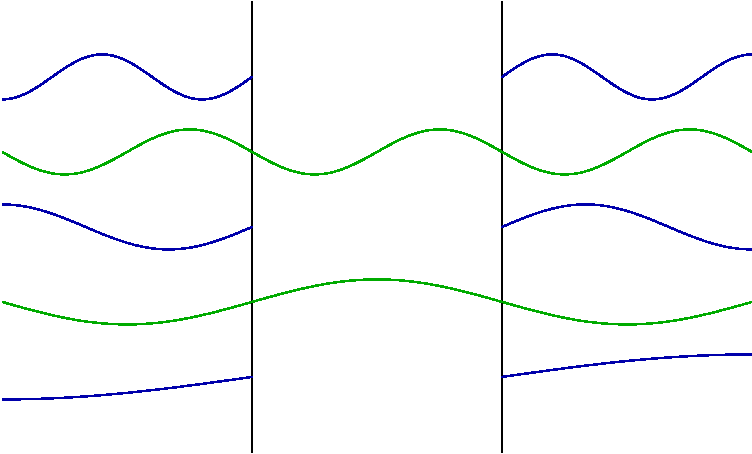
\includegraphics[width=10cm]{fig/intro/twoplanes_wave}
\caption{Sketch of allowed modes between perfectly conducting plates.}
\label{fig:Casimir_sketch}
\end{figure}

The theory was extended by Lifshitz to describe forces between dielectric half-spaces~\cite{Lifshitz1956}.
In the limit of dilute bodies the Casimir-Polder results for interacting atoms are recovered.  
This was further expanded on by Dzyaloshinskii~\etal\cite{Dzyaloshinskii1959,Dzyaloshinskii1961} who
showed the connection between Casimir force and the pair-wise van der Waals potentials.  
This work is nicely reviewed by McLachlan~\cite{McLachlan1963, McLachlan1963a}.  


\item Wall-Wall Effective action.

\begin{figure}
\centering
\begin{fmffile}{wall-wall}
\begin{fmfgraph}(50,30)
 \fmftop{t0,t1,t2,t3}
 \fmfbottom{b0,b1,b2,b3}
 \fmf{fermion,tension=0}{t1,v1}
 \fmf{fermion,tension=0}{t2,v3}
 \fmf{fermion,tension=0}{b1,v2}
 \fmf{fermion,tension=0}{b2,v4}
 \fmffreeze
\fmf{photon,tension=0}{v1,v3}
\fmf{photon,tension=0}{v2,v4}
\fmf{fermion,tension=0}{v1,v2}
%\fmf{fermion,tension=0,left}{v2,v1}
\fmf{fermion,tension=0}{v3,v4}
%\fmf{fermion,tension=0,right}{v4,v3}
\end{fmfgraph}
% \begin{fmfgraph}(50,30)
%  \fmftop{t0,t1,t2,t3}
%  \fmfbottom{b0,b1,b2,b3}
%  \fmf{phantom}{t1,v1}
%  \fmf{phantom}{t2,v3}
%  \fmf{phantom}{b1,v2}
%  \fmf{phantom}{b2,v4}
%  \fmffreeze
% \fmf{photon}{v1,v3}
% \fmf{photon}{v2,v4}
% \fmf{fermion,tension=0}{v1,v2}
% \fmf{fermion,tension=0,left}{v2,v1}
% \fmf{fermion,tension=0}{v3,v4}
% \fmf{fermion,tension=0,right}{v4,v3}
% \end{fmfgraph}

\end{fmffile}
\caption{Casimir Energy in terms of fundamental QED processes.  Electrons are considered bound within their respective media.}
\end{figure}

\item Picture of Electrons interacting with EM field.
  Effective action at some loop order in basic QED.
  Makes contact with fundamental physics.
  Can then make sense of limits in which we are operating.
  Doing perturbation theory on QED.
  $\epsilon$ is linear response of medium to EM field, and working to leading order in $\epsilon$.
  Amounts to $\order(\alpha_0^4)$ diagram for QED with electrons bound via nuclear potential.   (Again, very low energies).
\item Assuming electrically neutral
\item Far from atomic separations, so continuum approximation acceptable.
\end{itemize}



% As pointed out by Rosa~\etal~\cite{Rosa2010}\comment{right paper?}, 
% the Lifshitz theory is a classical stochastic electrodynamics theory,
% which attributes the fluctuations as thermal fluctuations of the medium.  
In somewhat later activity from this school, Barash and Ginzburg further extended this work to 
discuss the finite temperature effects, dissipation and the relation to the
microscopic details of the medium~\cite{Barash1975}.  

%\begin{itemize}
% \item Historically earlier, London applied interaction dipoles in QM perturbation theory.
% \item Casimir-Polder looking at colloidal suspensions, included retardation due to the finite speed 
%     of light.  
% \item As a matter of nomenclature we will refer to the whole range phenemena as the Casimir effect,
% in particular referring to the interaction between macroscopic bodies.  
% while referring to atom-surface effects as Casimir-Polder effects.  The near-field limit
% passes over to an instantenous dipole interaction,and will be referred to as the van der Waals regime.  
% Distinguish between atomic and macroscopic forces, and in different distance regimes.
% \item Ultimately, same physical origin.  
%\end{itemize}

% This example calculation is also carried out in the initial chapters of Ref.s~\cite{Milton2001,Bordag2009,Dalvit2011}.

% As QED calculation, the Casimir energy is formally divergent and must be renormalized in order to
% make physical predictions. 
%  In our case, we typically energy differences when one of the bodies is 
% removed to spatial infinity.
%   In some cases, like spheres the renormalization must be carried out more carefully.  
%   In those cases, the formally infinite parameters renormalize the physical parameters of the model~\cite{Milton2001}.  

\subsection{Physical Interpretation}

\begin{itemize}
  \item A number of interpretations.  Can attribute fluctuations to medium or fields.  
    van der Waals fluctuating dipoles vs Casimir fluctuating EM fields.  
    Atom/Bodies emitting and re-absorbing virtual photons.  
  \item Zero-point energy.  
  \item Clearest physical picture is effective action from long-wavelength EM fluctuations 
    interacting with matter.
  \item Emphasizes connection to underlying physics.  
\end{itemize}



\subsection{Distance and Energy Scales}

\begin{itemize}

  \item Casimir energy at $1\mu m$.  Take a dipole of 1 Debye.    
    Compare with 
  \item Casimir pressure  at $1\mu m$
  \item Cite Milonni for capacitance calculation.  


We can estimate typical distance scales by considering the dominant 
resonances of the medium, and the thermal wavelength.
  So the Casimir force is typically then important at distances below the
 transition wavelength which is usually around $1\mu m$.    

\item Considering long-wavelength approximation to medium.  Typically interested in forces
    on the micron-nanometer scale.  Above a few microns the force is too small to observe,
    while below a nanometer the forces are too strong to reliably isolate the atom 
    and the continuum approximation starts to break down.  

\item The typical energy scale can also be estimated.
  If we consider an atom with a static polarizability of 
$\comment{polarizability}$, at a distance of $1\mu m$, we find the Casimir-Polder potential is \ldots. 

For macroscopic bodies we can compare the Casimir energy for perfect 
metal conductors at a distance $d$ to the energy stored in the capacitance.
  Note that we compute an energy per unit area.  
\comment{Milonni makes the comparison to capacitance, \cite{Milonni1994}}

The Casimir energy per unit area is $\frac{\hbar c\pi^2}{240 d^3}$, while the voltage for a parallel plate capacitor is.
\begin{shaded}
\begin{itemize}
\item Capacitance is $V=Q/C$.  
\item $C = \epsilon_0 A/d$.  
\item Energy is $\frac{1}{2}CV^2=\frac{Q^2}{2C} $
\end{itemize}
\end{shaded}

\item Casimir forces are short ranged forces and decay away quickly --- for example the 
  London dispersive force between two atoms decays as $d^{-6}$.  In comparison
    the Coulomb potential between charged particles is behaves as $d^{-1}$,
    where $d$ is the particles separation.  While the Coulomb potential
    can be neglected for neutral atoms, it is much more relevant for macroscopic bodies.  
    
  For macroscopic bodies, the decay is slower, since we can roughly think of
 integrating up the contributions from all of the constituent atoms.
  For Casimir energies, the energy decays as $d^{-3}$.  


\item Since the Casimir force is a broadband phenomenon, it depends on the resonant frequencies 
    of the interacting media, such as the atomic polarizablitiies $\alpha(\omega)$ or the dielectric
    function $\epsilon(\omega)$.  Furthermore at nonzero temperature, there is a thermal wavelength,
    $\omega_T=\kB T/\hbar$.  
    Given the radiative nature of the Casimir effect, there is a factor $e^{i\omega d/c}$ weighting the 
    frequency integrals.  This contributes most when its exponent factor is order one.  
    The Lifshitz integral can be approximated in differing regimes.  

    In the near-field or van der Waals regime, the media are assumed to closer than the 
    resonant wavelength of the media $d\ll \omega_A/c,\omega_M/c$, the exponential factor 
    is unity, and each frequency contributes equally.  In essence, the interaction is an instantaneous 
    dipole interaction between the media, which inspires the name.    

    The so-called Casimir-Polder regime occurs when the atoms are much further than a resonant wavelength 
    $d\gg \omega_A/c,\omega_M/c$,
    in which case the dominant contributions come at zero frequency, and the functions can be approximated
    with their static limit.  This far-field regime typically makes the potential decays more quickly.  

    Even further away from the bodies is the thermal regime $d\sim \omega_T/c$, where the real photons excited by the 
    thermal field contribute significantly.  In this regime the field decay is typically slower as $E\sim d^{-3}$,
    the same as the near-field van der Waals regime.  
    \comment{table?}

\end{itemize}

\section{Summary of Casimir Experiments}

The Casimir effect has been measured in experiments, both for macroscopic bodies and atoms.
Beyond its interest as a fundamental quantum effect, the Casimir force is also important 
in designing novel physical devices for both atoms.

%Lamoreaux
\subsection{Casimir}
An early indirect measurement was liquid Helium flowing up the walls of a container.  
Lifshitz and co-workers applied the Casimir pressure to explain the phenomenon of liquid helium
flowing out of a jar.  The presence of the liquid helium crawlign up the surface reduces the Casimir energy,
so the liquid helium experiences an attractive pressure up the walls.  

While Casimir predicted an attractive force between neutral metal bodies in 1948,
it was only precisely measured in 1997 by Lamoreaux~\cite{Lamoreaux1997}.   
%Lamoreaux's work spurred a large amount of experimental and theoretical work.  
This experiment measured the Casimir force between a sphere above a metal plate,
and measured the force by detecting the change in capacitance of the arrangement.  
This landmark experiment was closely followed by measurement by Mohideen\etal\cite{Mohideen1998}
using an atomic force microscope to measure the force in a sphere-plate geometry.  
The Casimir force has also been directly measured in a nanoelectromechanical (NEMS) system 
by Chan~\etal~\cite{Chan2001}.  In this case, the Casimir force is detected by the modification it
makes to the frequency of a torsional oscillator suspended above a plate.  

The sphere-plate geometry has the experimental advantage of removing the need to carefully
align the metal plates. Given the strength of the Casimir force it is hard to keep the plates exactly parallel,
and separate, which is something that dogged early attempts to measure the Casimir force.
Despite the aforementioned difficulties, Bressi\etal measured the Casimir force between parallel plates~\cite{Bressi2002}.  
\comment{Lower precision?}

The Casimir force is also important in applications of microelectromechanical systems (MEMS), 
as a source of stiction~\cite{Tas1996, Serry1998, Buks2001}.  This is particularly important
in free standing structures such as nano-oscillators.  
Given the Casimir force is an attractive potential, if parts of the device get too close to the substrate
they will permanently stick to one another, leading to device failure.  

Precisely measuring such a small force requires careful calibration of the measurements 
and removing systematic effects.  Two of the primary experimental errors are due to 
patch potentials, and surface roughness.  The patch potentials are localized surface 
charge distributions, which due to the longer range Coulomb interaction swamp the weaker
Casimir force.  Surface roughness reflects the fact the surfaces are not perfectly smooth,
and as such the exact distance between bodies is not clear.  While the roughness can be taken into
account in theory, the surface must also be carefully characterized.  Reviews of these and other 
difficulties are available from

\subsection{Casimir-Polder}
%Skip over names?  
The Casimir-Polder force has been measured in the context of atomic beams, cavity QED, and 
Bose-Einstein condensates.  

\begin{itemize}
  \item 
    The first attempts at directly measuring the Casimir-Polder force used atomic beams 
    near surfaces.  
    Sukenik~\etal made the first modern attempt to measure the Casimir-Polder force~\cite{Sukenik1993}.
    Their experiment passed a hot beam of atoms through an optical cavity and attempted to detect
    the effect by the small phase-shift induced on the atoms.  Unfortunately, their measurement 
    was not definitive.
    More recent experiments by Perreault~\etal\cite{Perreault2005}, and Lonig~\etal\cite{Lonij2009} succed in measuring
    the Casimir-Polder force with atomic beams.  These experiments passed an atomic beam past grating and 
    detected the phase-shift by atom interometry.  % These experiments act as precision tests of the theory,
    % and found that the first principles calculations based on perturbation theory are less successful
    % than an effective description informed by experimental data.  

% \item Cronin \cite{Perreault2005,Lonij2009}  Atom interferometry experiments for atoms near gratings.
%   Pass hot atomic beam through gratings.  Useful as precision tests of theory.  
%   Typically find first-principles theory based on perturbation not working as well,
%   as effective descriptions which rely on experimental computations.  
\item 
    The Casimir-Polder effect has also been observed in the context of a Bose-Einstein Condensate (BEC)
    of ultra-cold atoms~\cite{Harber2005,Obrecht2007}.  The BEC allows for precise distance control,
    and can be used in atom interferometry to detect small phase shifts.    
    The atoms are confined to a harmonic trap, and can be brought near to a surface to probe the Casimir
    force.  The Casimir force acts to shift the oscillation frequency of the harmonic trap in a position
    dependent manner.  
    Furthermore, this technique was able to measure the Casimir force in the thermal regime, which
    is often difficult since the force is weak at those distance.  In this case it is easy to 
    vary the distance of the atoms from the surface from $1\mu m$ up to 10 $\mu m$ to observe
    the cross over between the Casimir-Polder and thermal regimes.

% Measured Casimir-Polder shift in Bose-condensed gas of ultra-cold atoms.
%   Harber\etal\cite{Harber2005} measured the shift in the oscillation frequency
%   of a Bose-Einstein condensate (BEC).  BEC used for enhanced signal, well localized.
%   Casimir force not relevant to coherent aspects of BEC.
  % Obrecht\etal\cite{Obrecht2007}Also measured force in the hard to measure thermal regime.  
  % Can easily vary distance of atom from surface from $1\mu m$ up to $10\mu m$ from surface.
  % Relate to lifshitz formula and cross-over.    

\item Quantum computing devices
    \begin{itemize}
      \item Quantum computing offers to make certain computation tasks (most notably factorising 
        large prime numbers) and simulation taks much more efficient.  
      \item Large push to develop scalable quantum devices in a number of model systems
        (NV centers, cold atomic gases).  Atoms provide excellent quantum memory, internal
        states are well isolated, controllable interactions via lasers.  
      \item In order to address each atom, and ensure strong interactions, some groups 
        ar developing microscopic dielectric waveguides to allow trapping, addressing and strongly interacting with a 
        single atom in a scalable manner~\cite{Alton2011, Hung2013, Goban2014}.  
      \item In designing these new devices it is essential to compute and account for the Casimir-Polder force
        the atom's experience when brought close to the dielectric surface.  
    \end{itemize}

    The Casimir-Polder effect is also important in the design of devices aiming to trap and interact
    with atoms near surfaces.  While ultra-cold atoms are very clean systems to work with for 
    studying and exploiting quantum effects, they are hard to minaturize and scale up.  In recent
    years there has been a concerted push to develop technology to regain the appealing features 
    of cold atoms in a scalable architecture. 
    One direction that has been pursued is the so-called atom-chip\cite{Folman2000,Schneider2003}, where atoms are 
    trapped near surfaces via a combination of lasers and magnetic fields from wires embedded in
    the surface.  The atoms are typically trapped within a micron of the surface.  
    In most applications the Casimir effect acts as a lower bound on how close bodies can be brought 
    to each other, which in turn limits the coupling strength and thus the speed of operation.  
    \comment{other work - books?}
    In addition, the Casimir force as been taken into account in design 1D atom traps 
    near a nanowire~\cite{Salem2010}.

    Another direction that has been pursued is strong coupling of atoms to light via cavity 
    quantum electrodynamics (QED).  While originally pursued with high-finesse Fabry-Perot optical
    cavities, this has since been exploring the use of dielectric waveguides

\item Antezza - chapters in Dalvit.  
% \item Kimble atoms near toroidal resonators.
%   Strongly Couple single atoms to optical field at single photon level.  
%   Apply to toroidal resonators, and dielectric waveguides.  
%   \cite{Alton2011}.
%   Atoms above 1D Microcavity \cite{Hung2013}
\item Atom-chips and atom-waveguids are attempts towards building scalable 
architecture for quantum computer using atoms.
Couple atoms to dielectric waveguides, and get stronger coupling (thus faster operation)
by moving atoms more closely to couple to evanescent field.  
\end{itemize}
Challenges:  Need to characterize surface over broad frequency range.
Need methods with converge well for all geometries.  

\subsection{Current experimental directions}
\begin{itemize}
\item Thermal casimir force
Sushkov\cite{Sushkov2011}.
Fight in literature over exact model used to describe metals at finite temperature.
Drude vs plasma model.  
 Lamoreaux favors Drude model, Capasso/Mohideen favours plasma model.
\item Repulsion (Cite Capasso experiment with bromobenzene).  Possibility of stable trapping
  if one could balance repulsion/attraction.  
 Metamaterials for repulsion.  (Can't work Rosa 2010/2011 since dielectric
  background dominates~\cite{Rosa2008})
  (Cite Vogel and Welsch chapter for Green function methods.  They cite 
  Feinberg and Sucher (1970) on pg 360 for repulsion)
  \item Search for repulsive forces as possible trapping (Motivation for this?)
  \item Can be found for magnetic media (but typically small).
    Metamaterials exhibit this for small range of frequencies.
    But Casimir broadband, and dielectric contribution ends up dominating.
    (\comment{ Cite Milonni on metametarials}.
    Sufficiently anistropic dielectric media (how anisotropic? \comment{Cite Milton})
    $\epsilon_1<\epsilon_3<\epsilon_2$ over a broad enough range of frequencies 
    \comment{Cite Lifshitz of liquid helium.
    Cite experiments, and note odd fluids.}.
    Geometries dependence (\comment{Cite reid paper on needle above hole}).
    
% Modifications to gravity on $1\mu m$ or $1mm$ scale.  Cite Lamoreaux 2000 Paper.  Gervaci?
% Yukawa type forces.  (Carrol's textbook on string theory dilaton.  
%  Subtract off Casimir force background.
%   Tino group.
%   Use Casimir shield with fairly thick gold to have same Casimir force, and thne vary the medium behind it.
%   Longer range gravity should lead to 
% Requires very careful measurements, on top of carefully extracting Casimir force.   

\item The Casimir force is also important for speculative searches for new physics on the millimeter to micron
scale~\cite{Dimopoulos2003, Bezerra2011}.  The new physics must be shortranged, and is typically modelled as 
a Yukawa potential, $V_{\text{Yuk}}=\alpha e^{-\lambda r}/r$.  
On this scale however, the Casimir effect is the dominant interaction, and must be 
carefully subtracted in an experimental procedure.  However, one can look for deviations from the expected 
power laws, which has been used to exclude regions of the parameter space for the hypothetical
Yukawa interaction~\cite{Lamoreaux1997,Obrecht2007,Bezerra2011}.  
Experiments searching for modifications of gravity typically employ a thin gold layer over
a density modulation.  The gold layer provides a common short-ranged Casimir interaction, while the 
a density modulation allows measuring variations due to gravity~\cite{Sorrentino2009, Geraci2015}.
Given the difficulties in cleanly measuring the Casimir force, this even more ambitious program has yet 
to yield results.  
\end{itemize}


% \subsection{Chemistry/Helium/Geckos?}

% \begin{itemize}
% \item Geckos use the Casimir force \cite{Autumn2002}.
% \item Military applications to mimic at human scale. Cite 2015 paper.   
% \end{itemize}

\section{Computational methods}

Describing this range of phenomena require that one handle material properties reliably, and with arbitrary geometries,
and possible anisotropies.  Typically working in long-wavelength approximation which neglects strong
forces binding bodies together.    

A common thread throughout these now classic computations is an emphasis on exactly solvable
geometries.  With the advent of modern experiments however, it is necessary to be able 
to compute the Casimir force in arbitrary geometries, with general material properties in order
to compare theory and experiment.  

\begin{itemize}
\item Experiments spurred development of theory.  
\item Prior methods relied on mode-function expansion of fields, which is only possible
for simple geometries.  
\item Theory must account for material properties.  Surface roughness.  
\item Need general methods, tend to result in numerical integrals.
\item Crudest method available is the proximity force approximation.  
\item Analytical theory based on green function methods.  (Russian school, McLachlan, Schwinger)
\item Scattering approach.  
\item Worldline method.  
\end{itemize}

\subsection{Proximity Force Approximation}

\begin{itemize}
\item The proximity force approximation (PFA) is an uncontrolled approximation to
the Casimir force between generally shaped objects.  
The PFA computes the Casimir force can be found by treating each infinitesimal segment
of the surfaces as if they were planes, and integrating the force between surface patches.
\item Find first use?  Lamoreaux mentions usage.  Derjaguin?\cite{Derjaguin1956}
\item Note problem with non-additivity. The PFA explicitly assumes that the force
can be found by adding up the pair-wise contributions from each surface patch.  
However, the Casimir force is a global phenomenon, and the total Casimir force
Useful if very limited curvature, or effectively approximate geometry as planar.  
\item Only attractive.  (real electromagnetic casimir forces have possibility of 
being repulsive, even if hard to realize in general.)
\item ever extended to include material properties?
\item Despite these limitations, the PFA is relatively straightforward to implement,
and functions as an order of magnitude estimate for the Casimir force.  In the limit
of vanishing curvature, the PFA converges to the correct Casimir force.  
\end{itemize}

\subsection{Green function methods}

\begin{itemize}
%\item Cite Lifshitz, Dzyaloshinski, Abrisokov.
\item Cite McLachlan~\cite{McLachlan1963}
\item Cite Schwinger~\cite{Schwinger1978, Milton1978}  Scalar green functions.  
\item Green tensor methods
\item Cite Barton
\item Cite Philbin(?)
\item Cite Vogel and Welsch
\item Green function equation
\begin{equation}
  \nabla\times\nabla\times G(\vect{x},\vect{x'}) + \frac{\omega^2}{c^2}\epsilon G(\vect{x},\vect{x'})  = \delta_{ij}\delta(\vect{x-x'})
\end{equation}
\item Energy expressions.  
\begin{equation}
  E_{CP} = \int_0^\infty ds \alpha_{ij}(is,\vect{x})G^{(S)}_{ji}(is,\vect{x},\vect{x})
\end{equation}
Focus on scattering part - renormalization.  $\alpha$ is atomic polarizability tensor,
 $G$ is electromagnetic Green tensor.  
 Evaluate at imaginary frequency. Note fully quantum theory, can account for atomic transitions.
\item Definition of $\alpha$,$G$ in terms of eigenfunctions, field modes.  
\begin{equation}
  \alpha_{ij} = \sum_n\sum_m \frac{\langle E_n | d_i|E_m\rangle \langle E_m| d_j|E_n\rangle}{E_m-E_n}
\end{equation}
\item Calculations correspond to given order of perturbation theory in QED hamiltonian.  
\item Finite temperature.  
\end{itemize}

\subsection{Scattering Approach}

The scattering approach is currently the only general method of computing 
electromagnetic Casimir forces in general media.  The essence of the scattering method 
is encodes the presence of material bodies by the electric field they scatter.  

While originally developed as an analytical
technique, the scattering method has also been converted to an efficiency numerical method.  

It has been explored as an analytical technique,
and further converted to a form 
\begin{itemize}
\item EM field depends on scattered field.  Encoded in reflection matrices
which are related to how EM field scatters from a given surface.  
\item Developed as analytical technique, and developed into general purpose numerical technique.
Numerous authors contributed over decades.
\end{itemize}

\begin{itemize}
  \item Developed as general method, for scattering between basis modes.  
    Initially used with analytical mode expansions.  Can also use finite element basis,
    much more adapted to arbitrary bodies.  
\item Physical picture is fluctuating currents on bodies.  Interact via EM field.
  Can use Green function as if dielectric suffused all space.  
Surface-Integral Equations (SIE) and Green's theorem relate surface integrals.  
\end{itemize}

\begin{itemize}
\item Cite Balian and Duplantier \cite{Balian1977, Balian1978}.
\item Cite Lambrecht and French collaborators
  \cite{Lambrecht2006, MaiaNeto2008,Canaguier-Durand2012}
%\item Cite Milton
\item Physical Picture based on generalized Green theorem from 
  SIE~\comment{Stratton}\cite{Stratton1941}.
\item Comment on Emig/Buscher showing you can use homogenous green function.
  Relation to Green's theorem.
\item Cite Emig,Jaffe,  and others for initial analytical techniques.  Relies on Green theorem.
\cite{Emig2004, Emig2007, Rahi2009}
\cite{Kenneth2006}
  Note use of existent analytical methods and similarities to existent 
  numerical FTDT techniques on earlier papers.  
  \cite{Rodriguez2007,Rodriguez2007a, Rodriguez2009}
\item Cite Johnson/Reid for numerical progress.\cite{Reid2009,Reid2011, Reid2013}.
\item Note success, applicability.  \comment{Cite experimental tylenol pill paper}
\end{itemize}

\subsection{Modern Directions}

\begin{itemize}
  \item Non-additivity of forces:  Reference for this?  What is the typical scale of the correction for non-additivity?

  \item Search for repulsive forces

  \item Casimir force important for stiction.
  \item Attracts atoms, sets lower bound for how close you can get particles together.
\item Dynamical Casimir effect/Unruh Effect?
    \item Accelerating plate creates photons.  
  \end{itemize}


\section{Scalar Worldline Casimir Energies}

The worldline method is an alternative method for computing Casimir energies.
  The worldline method was initially developed as an alternative method for 
carrying out QFT calculations in terms of particle 
mechanics~\cite{McKeon1993, Strassler1992,Schubert2001}.
  In particular the quantum effective actions can be computed in terms of
 the suitable dynamics of a quantum particle.
\comment{Other references - was one contemporaneous with Strassler? Bern-Kosower}

The basic insight is that for one loop effective actions, 
the field path integral calculation can be recast in terms of the particle path
 integral for particles travelling in closed space-time loops.
  This is quite similar to the scalar electrodynamics Feynman explored
 in his Ph.D thesis~\cite{Feynman1942, Brown2005}
\comment{Seems to actually be his 1950 QED paper RE Schubert2001}.
  Higher order loop calculations can also be carried out with more particles, 
and gauge fields can also be treated~\cite{Schubert2001}.
  For example, the worldline method has been used to compute relativistic
 field effects for QED such as the Lamb shift~\cite{Schmidt1995}, and as a numerical algorithm~\cite{Mazur2014}.

The worldline method is heavily based on Feynman's path integral method~\cite{Feynman1948,Feynman1965}.

Our primary interest in the worldline method is for computing Casimir energies, 
which was first used to compute scalar Casimir energies by Gies~\etal~\cite{Gies2003,Gies2006, Gies2006a}.
 While the initial work focused on the zero temperature limit, 
the worldline method has also been extended to finite temperatures~\cite{Klingmueller2008}.
  This has also been used to study the torsion of inclined planes~\cite{Weber2009},
 and planes and spheres and planes and cylinders~\cite{Weber2010, Weber2010a}.  

% We will briefly introduce the method here, and discuss the method at 
% length in Ch.~\ref{ch:scalar_worldlines}.  
Let the action for the scalar field be given by 
\begin{equation}
  S = \int_0^T dt \int d^3x \left[ (\partial_t\phi)^2-(\nabla\phi)^2-V(\vect{x},t)\phi^2\right],
\end{equation}
where $V(\vect{x},t)$ defines the surfaces of the objects we wish to compute
 the Casimir energy between.
  The potential is typically chosen to be $V(\vect{x},t)=\lambda\delta[\sigma(\vect{x})]$,
 where $\sigma(\vect{x})=0$ defines the surfaces.
  In the limit $\lambda\rightarrow\infty$ the potential enforces Dirichlet boundary conditions 
  on the surfaces of the bodies.  In certain geometries this recovers electromagnetic 
results assuming the surfaces are idealized perfect conductors.  

We can compute the partition function for the field by Wick rotating to
 imaginary time (or finite temperature), where the partition function is now given by 
\begin{equation}
  Z = \int D\phi \exp\left\{-\int_0^T dt \int d^3x 
    \left[(\partial_t\phi)^2+(\nabla\phi)^2+V(\vect{x},t)\phi^2\right]\right\},
\end{equation}
The Gaussian integration over fields can be formally carried out as a functional determinant.
  In order to compute the energy we need the logarithm of the partition function,
 and various derivatives of it.
  The end result of these manipulations is that the renormalized energy can be written as 
\begin{equation}
E_{\text{scalar}} = \frac{\hbar c}{(2\pi)^{D/2}}\int_0^\infty \frac{d\cT}{\cT^{1+D/2}}
 \int d\vect{x} \dlangle e^{-\cT\langle V\rangle} -1\drangle,
\end{equation}
where $\cT$ is the loop ``time'' and governs the extent of the loops,
 $\vect{x}_0$ is the loop starting point, $\dlangle \cdots\drangle$ denotes 
an ensemble average over closed Gaussian random walks, 
and $\langle\cdots\rangle$ denotes the average of a quantity around the loop.  

\begin{figure}
\center
\includegraphics[width=10cm]{fig/intro/hit_strong_coupling}
\caption{Upper loop touches both objects and will contribute to Casimir energy.  Lower loop only touches one body, and does not contribute to Casimir energy.}
\end{figure}


\begin{itemize}
%\item Cite Schubert~\cite{Schubert2001}, Strassler~\cite{Strassler1992} on general worldline
% \begin{itemize}
% %\item Summarize Strassler.  Can compute QFT effects from worldline path integrals.  
% % \item One loop effective actions can be described as single-particle worldline path integrals.  Can apply for higher order loops, and gauge fields, Cite Schubert.    
% % \item Cite QED at one loop order paper.  Get same results.  
% % \item Note similarity to Schwinger's trick for handling loop integrals in QED.  T is Schwinger's proper time.  
% \end{itemize}
%\item Cite QED Worldline paper on numerics?
\item Cite Schaden applying to pistons\cite{Schaden2009}
\item Figure showing loops.  
\item Advantages
  \begin{itemize}
  \item Algorithm is geometry independent, and no spatial grid.
  \item parallelizable.  Computation time scales as one /resources.  
  \end{itemize}

\item Shortcomings
\begin{itemize}
  \item A scalar, not vector electromagnetism.
  \item Idealized boundary conditions.  
\end{itemize}
  
\end{itemize}


Thus far the worldline method has only been developed for scalar fields, 
without direct application to electromagnetic Casimir problems, 
other than for some speculation~\cite{Aehlig2011}.
  Currently, the potentials reflect the imposition of Dirichlet boundary 
conditions on the surfaces of the bodies, rather than a physical dielectric.
   In our work we will show how to incorporate the dielectric explicitly, 
and show how in simple geometries a new version of the scalar theory applies
 to electromagnetic problems.  

Quantization of the electromagnetic field inside dielectric has been considered
 by a number of authors.  
Some care is required to handle dispersion, since the Kramers-Kr\"onig relations
 imply this also requires dissipation \comment{citation?}.  
This is typically handled by coupling the electromagnetic field to an idealized
 medium, and coupling the medium to a bath of oscillators that models
 dissipation~\cite{Huttner1992,Dung1998}.  

Bechler has carried out path integral quantization for a harmonic medium 
including dispersion, and shown agreement with previous results in terms 
of noise operators~\cite{Bechler1999}.  
The primary results were the form of the propagator, 
rather than computations exploiting the propagator.
  There has been some work attempting to develop path integral quantization of
 the field inside dielectric neglecting dispersion~\cite{Bordag1998}.
  Unfortunately, these results are hard to interpret given that the non-physical
 degrees of freedom for the field do not cleanly decouple, as opposed to the 
usual situation in free space QED.
  The primary focus here was to explore the divergence structure of the theory
 via the Heat Kernel expansion, which corresponds to the small time expansion
 of a worldline path integral.
  We choose to avoid this issue by focusing on improved scalar models, 
that also correspond to the physical degrees of freedom for the field in certain geometries.  

Others have made models in the static limit by ignoring the fluctuations in the field,
and focusing purely on the electrostatic energy.
 Similar functional determinants to worldline methods are found,
 and are evaluated explicitly using a spacial grid~\cite{Pasquali2008}.  

% \section{Copied}
% \label{ch:scalar_worldlines}
% \begin{itemize}
% \item Cite Schubert~\cite{Schubert2001}, Strassler~\cite{Strassler1992} on general worldline
% \comment{Other references - was one contemporaneous with Strassler?}
% \begin{itemize}
% \item Summarize Strassler.  Can compute QFT effects from worldline path integrals.  
% \item One loop effective actions can be described as single-particle worldline path integrals.  Can apply for higher order loops, and gauge fields, Cite Schubert.    
% \item Cite QED at one loop order paper.  Get same results.  
% \item Note similarity to Schwinger's trick for handling loop integrals in QED.  T is Schwinger's proper time.  
% \end{itemize}
% \item Cite QED Worldline paper on numerics?
% \item Cite Gies papers~\cite{Gies2003,Gies2006, Gies2006a} (all of them!) note work on thermal/geometry~\cite{Klingmueller2008,Weber2009, Weber2010}
% \end{itemize}

% In this chapter we will review prior work on the worldline method, translated to our terminology
% and conventions.  We will derive the method, and discuss its advantages and shortcomings.  

\section{Partition Function to Worldline path integral}

\begin{itemize}
\item Intro
We consider a scalar field coupled to a background potential $V(\vect{x},t)$.  This potential
embodies the location of the bodies we are considering.  Starting from the classical action,
we will derive the Hamiltonian for the fields, and then compute the quantum partition function.  
The partition function can be written as a path-integral, which is readily evaluated as a functional
determinant.  Ultimately we want the free energy, which can be further converted into a path integral
for a fictitious single-particle.  This single-particle path integral forms the basis of the numerical
world line method.   

\item Lagrangian - Hamiltonian
The Lagrangian for the scalar field is
\begin{equation}
  L := \int d^3x \left[ \frac{1}{2}(\partial_t\phi)^2-\frac{1}{2}(\nabla\phi)^2-V(\vect{x},t)\phi^2\right].
\end{equation}
In prior work, the potential $V(\vect{x},t)$ encodes the locations of the interacting bodies, with 
definition
\begin{equation}
  V(\vect{x}) = \lambda \sum_r \delta[\sigma_r(\vect{x}-\vect{R}_r)],
\end{equation}
    where $\lambda$ is the coupling constant, $\sigma_r(\vect{x})=0$ marks the locations of the surfaces, 
    and $\vect{R}_r$ marks the center location of each body.  The coupling constant $\lambda$ 
    is taken to infinity, which corresponds to imposing Dirichlet boundary conditions on the surfaces.

% The conjugate momentum to $\phi$ is given by
% \begin{equation}
%   \Pi := \frac{\delta \cL}{\delta(\partial_t\phi)} = \partial_t\phi,
% \end{equation}
%     where $\frac{\delta}{\delta f(t)}$ denotes the functional derivative w.r.t. $f(t)$.    
% The Hamiltonian can then be easily found,
% \begin{align}
%   H := \int d^3x\,\Pi\partial_t\phi -  L\\ 
%   = \int d^3x\,\bigg[\frac{\Pi^2}{2} + \frac{1}{2}(\nabla\phi)^2 +V(\vect{x},t)\phi^2\bigg].  
% \end{align}
% We are now in a position to quantize the field by promoting the fields to operators, 
%     $\phi\rightarrow \op{\phi}, \Pi\rightarrow\op{\Pi}$.
% The fields can be promoted to operators with equal-time commutation relations
% \begin{equation}
%   [\op{\phi}(\vect{x},t),\op{\Pi}(\vect{x'},t)] = i\hbar \delta(\vect{x}-\vect{x'}).
% \end{equation}
% In exactly analogous fashion to quantum mechanics, the overlap between states is given by 
% \begin{equation}
%   \langle \phi|\Pi\rangle = \exp\bigg[\frac{i}{\hbar}\int d^3x \phi(\vect{x})\Pi(\vect{x})\bigg].
% \end{equation}
    
    We can compute physical quantities of interest such as Casimir energies and forces
    by taking suitable derivatives of the free energy.  The free energy $\mathcal{F}=-\kB T \log Z$,
    is in turn given by the partition function $Z$.  \comment{Cite Brown, Altland-Simons}

The field partition function is 
\begin{equation}
  Z = \tr[ e^{-\beta\op{H}}] = \int d\phi \langle \phi| e^{-\beta \op{H}}|\phi\rangle,
\end{equation}
where we have evaluated the trace over the complete set of field states.  In classic path-integral
fashion the exponential operator can be split into $N$ pieces, and resolutions of the identity
in both fields and conjugate-momentum fields can be inserted between each piece.  

% \begin{align}
%   Z &= \int d\phi_0\prod_{n=1}^N d\phi_n \langle \phi_n| e^{-\Delta \beta \op{H}}|\Pi_n\rangle
%   \langle\Pi_n| \phi_{n-1}\rangle
% \end{align}

After integrating out the momentum fields, the partition function can be written as 
\item Euclidean Path integral (Generating Function) 
\begin{equation}
  Z = \int D\phi \exp\left\{-\int_0^{\hbar\beta c} d\tau \int d^3x 
    \left[ \frac{1}{2}(\partial_\tau\phi)^2+\frac{1}{2}(\nabla\phi)^2+V(\vect{x})\phi^2\right]\right\}.
\end{equation}
The functional integral over $\phi$ is Gaussian and can be formally evaluated immediately as a 
functional determinant, since the differential operator is positive operator.  
Some care is required in regularizing such infinite determinants.  
This is done in analogy with finite dimensional Gaussian integrals.  
We can consider treating the fields as only being evaluated on a finite lattice of space-time points, 
with the lattice also having a finite extent which bounds all bodies.  We will then take the limit of 
arbitrarily large volume, and lattice resolution at the end.  The gradient operators 
can be treated via their finite difference approximations, which can be thought of as sparse matrices.  

% For a single real Gaussian integral, one can evaluate it as
% \begin{equation}
%   I_1=\int dx e^{-\alpha x^2} =\sqrt{\frac{\pi}{\alpha}}.
% \end{equation}
% Let us now consider the multidimensional Gaussian integral
% \begin{equation}
%   I_2=\int \prod_{j=1}^Ndx_j e^{-\vect{x}^T A \vect{x}},
% \end{equation}    
% where there is an implicit sum over $i,j$, and $A$ is a positive matrix, i.e. all of $A$'s eigenvalues $\alpha_j$ 
% are positive.
%     The Gaussian integral can be readily evaluated by changing integration variables $\vect{x}$ to the amplitudes of the 
%     eigenvectors of $A$, $\vect{y}$ via an orthogonal transformation $O$,
%     \begin{equation}
%       \vect{x} = O\vect{y}.
%     \end{equation}
%     The Gaussian integral can be evaluated as
%     \begin{equation}
%       I_2 = \int \prod_{j=1}^N dy_j e^{-\alpha_jy_j^2} \propto \left[ \prod_{j=1}^N\alpha_j \right]^{-1/2}
%       = {\det}^{-1/2} A.
%     \end{equation}
%     \comment{(Cite Srednicki or Brown for their chapter on Gaussian integrals)}
In an analogous fashion, one can formally evaluate the partition function path integral as a 
functional determinant, 
\begin{equation}
  Z \propto {\det}^{-1/2}\left[-\frac{1}{2}\partial_\tau^2-\frac{1}{2}\nabla^2+V(\vect{x})\right].
\end{equation}
Note that the original computations for the worldline method stressed computing the quantum effective
action for the scalar field.  This yields essentially the same expression.  

The free energy for the interacting field can be written as 
\begin{equation}
  \mathcal{F} = -\kB T\log Z = \frac{1}{2}\kB T \log\det[-\frac{1}{2}\partial_\tau^2-\frac{1}{2}\nabla^2+V(\vect{x})].
  \label{eq:free-energy-det}
\end{equation}
As it stands this expression is divergent, however we will renormalize by subtracting off the 
same expression with the bodies removed to spatial infinity.  Physically this corresponds to 
computing energy differences between different configurations.  The renormalization also cancels off 
the constant normalization factors.  

The free energy can now be converted into a single-particle path integral via some formal 
manipulations.  First we will use the identity $\log\det A=\tr\log A$, which can be readily
verified for positive finite matrices.  
\begin{align}
  \log\det A &= \log\prod_j \alpha_j%\nonumber\\
  =\sum_j \log\alpha_j%\nonumber\\
  = \tr\log A,\label{eq:log-det}
\end{align}
    where we used the facts that the trace and determinant of a matrix are given by the sum
and product of its eigenvalues respectively. \comment{Check Kirsten/Vassilevich for better argument/citation}
Furthermore, we will use the integral representation of the logarithm,
\begin{equation}
  \log A -\log B= -\int_0^\infty \frac{d\cT}{\cT} (e^{-A\cT} - e^{-B\cT}).\label{eq:integral_log}
\end{equation}
This expression also relies on a difference of terms to cancel out divergent terms at $T=0$.  The 
earlier renormalization by subtracting off the vacuum energy provides exactly this subtraction. 

By applying Eqs.~(\ref{eq:log-det}) and (\ref{eq:integral_log}) to free energy~(\ref{eq:free-energy-det}),
 the renormalized free energy can be rewritten as
\begin{equation}
  \mathcal{F}-\mathcal{F}_0 = -\frac{\kB T}{2}\int_0^\infty \frac{d\cT}{\cT}
  \tr\Big[e^{-(\partial_\tau^2+\nabla^2)\cT}\big(e^{-\cT V(\vect{x})}-1\big)\Big].
\end{equation}
    


\item Worldline path integral
  \begin{equation}
    F = - \int \frac{dT}{T^{1+D/2}} \dlangle e^{-\cT\langle V\rangle} - 1\drangle,
  \end{equation}
  where $\cT$ is the loop proper time, $\langle V\rangle$ is the average of the potential around a particular loop, and $\dlangle\cdots\drangle$ denotes an ensemble average over Brownian paths.  
\item Typically take $V = \lambda\delta[\vect{x}-\sigma(\vect{x})]$, where $\sigma(\vect{x})=0$ is a function describing the surfaces.  In the limit $\lambda\rightarrow\infty$ this amounts to enforcing Dirichlet boundary conditions on the fields at the surfaces.  
\end{itemize}

    \section{Numerical method}
    \section{Deficiencies of the scalar method}
\begin{itemize}
\item Cite Schaden applying to pistons\cite{Schaden2009}
\item Figure showing loops.  
\item Advantages
  \begin{itemize}
  \item Algorithm is geometry independent, and no spatial grid.
  \item Parallelizable.  Computation time scales as inversely with resources.  
  \end{itemize}

\item Shortcomings
\begin{itemize}
  \item No coupling of photons to medium.
  \item A scalar, not vector electromagnetism.
\end{itemize}
  
\end{itemize}


\begin{shaded}
  The presence of $\delta(\vect{x}_N-\vect{x}_0)$ leads to an overall normalization constant $(2\pi\cT)^{-(D-1)/2}$.
  This follows either from Hormander's argument, that 
  \begin{equation}
    \int d^nx\, \delta[h(\vect{x})]f(\vect{x}) = \int_{h^{-1}(0)} dS\,\frac{1}{|\nabla h(\vect{x})|}f(\vect{x}),
  \end{equation}
where $S$ is defined as the surface satisfying $h(\vect{x})=0$, and 
$|\nabla h(\vect{x})|=\sqrt{\sum_k \left(\frac{\partial h}{\partial x_k}\right)^2}$.
  In our case, we are restricting a sum of $N$ Gaussian integrals to have zero total.
  If we define the increments $d\vect{x}_n = \vect{x}_{n+1}-\vect{x}_n$, then the loop constraint is $\delta(\sum_{k=0}^{N-1} \vect{x}_k)$.
  If we account for the remaining normalizations of the $\vect{x}_n$ integral, then the normalization for the loop path integral is $\sqrt{2\pi\Delta \cT N} = \sqrt{2\pi\cT}$.  
\footnote{See pages 826-828 of Dan's notes.}
\end{shaded}


\section{Continuous Quantum Measurements}

Describe open quantum systems, and include information from continuous measurements. 
\begin{itemize}
  \item 
\end{itemize}


\subsection{Quantum Trajectories}

\begin{itemize}
\item Quantum measurements are inherently probabilitistic.  
\item Thus, sequences of measurements are also inherently random.  
\item Greater experimental control means we can now probe isolated quantum systems repeatedly and see how they evolve.  
\item Move beyond simple projective measurements, which cannot describe things like position measurements.
\item To describe continuously weakly probing a system, also use stochastic processes as part of
 numerical simulation strategy.
\item Quantum tajectories correspond to monitoring a quantum system (like an atom) via a probe,
 for example shining light on the atom. \cite{Carmichael1993}
\item Simulated trajectories are possible trajectories a system could trace out as we observe.
  Also given a particular measurement record, they correspond to our best estimate of the current state of the system.  
\end{itemize}



\begin{itemize}
\item Cite Carmichael Rice JOSA paper~\cite{Carmichael1989}
\item Carmichael 1991 ~\cite{Carmichael1991}
\item Open Systems approach to Quantum Optics\cite{Carmichael1993}
\begin{itemize}
\item Motivated by photodetection, and modelling experiments developed a new approach to open systems.  
\item Sample trajectories then correspond to actually results.
\item Naturally fits Bayesian framework for interpretation of quantum state.  
\end{itemize}
\item Cite Marte, Zoller, Parkins, Gardiner (MCWF)  \cite{Dalibard1992,Dum1992,Gardiner1992}

\item Cite Holland ~\cite{Holland1996}, Meystre~\cite{Greenwood1997}.
  Applied to position measurements of atoms by detecting photons.
  Detection of photons localizes atoms.  
\item Control Theory.~\cite{Wiseman1993}  Cite Wiseman book
\begin{itemize}
  \item Continuously monitoring system to implement closed-loop feedback control.  
\end{itemize}
\item Quantum Chaos
\begin{itemize}
  \item Idea of exploring quantum-classical transition.
  Strong measurement is more classical.
  Can extract Lyupanov exponents for diverging trajectories.
  \cite{Bhattacharya2000,Habib2002,Habib2006}
  \cite{Scott2001}
  \item Describe 
\end{itemize}
\item Advantages:
\begin{itemize}
  \item Computationally efficient as simulating wave functions.
  Take ensemble average at the end to get density matrix.  
  \item Natural form for feedback control and reconstructing trajectory.  
\end{itemize}
\item Comment: Relationship of measurement with state and process tomography?  Any?  

\item Warshawski and Wiseman.
  Can describe additional uncertainty by including classical Bayesian probabilities for each indistinguishable trajectory.
  Note thesis of J. Thorne describing model for EMCCD camera.
  Given number for each pixel have probabilities for each number of photons.
  Must then incoherently average over all possible detection histories consistent with measured record.
  \cite{Warszawski2002,Warszawski2003a,Warszawski2003b}
\item Also cover results for generalized measurement functions and 
somewhat surprising notion that particle reflects from a sufficiently
strong quantum measurement.
\end{itemize}

% \section{Thesis outline}

% We will cover some background material relating to field quantiuzation, thne proceed to develop the 
% relevant worldline path integrals.


% \begin{itemize}
% \item Background for path integrals, scalar worldlines, and EM field quantization.
% \item Cover 
% \item Analytical methods and computations in simple geometries.
% \item General method and numerical results.
% \item Shift to quantum trajectories.  
% \end{itemize}



%%% Local Variables: 
%%% mode: latex
%%% TeX-master: "thesis_master"
%%% End: 
